\documentclass[10pt,a4paper]{article}
\usepackage{graphicx}
\usepackage{placeins}
\usepackage{indentfirst}
\usepackage{enumitem}
\author{Bardi Bogdan}
\title{Polynomial Calculator}


\begin{document}
\begin{titlepage}
\centering

\includegraphics[width=0.5\paperwidth]{utcn.png}\par\vspace{5cm}
	{\huge\bfseries Order Management\par}
	\vspace{2cm}
	{\Large\itshape Bardi Bogdan\par}
	{\Large\itshape Group:30421\par}
	{\Large\itshape Year of Study: 2019-2020\par}
	\vfill
\end{titlepage}
\tableofcontents
\pagebreak
\section{Requirements}
The main goal of this assignment was to design and implement an application for processing customer orders for a warehouse.\par
To achieve the main objective I had to go through many different steps which will be thoroughly explained in the following chapters:
\begin{enumerate}
\item Analyzing use cases and the problem itself
\item Creating an UML Diagram and designing the necessary classes and data structures
\item Designing the user interface
\item Implementing the created designs
\item Creating unit tests
\end{enumerate}

\section{Problem Analysis}
In order to manage orders for a warehouse we need a database to store the necessary data to do so such as customers' name and address, product on stock, and the history of previous orders. To do so we use a relational database management system(RDBMS) such as MySQL or Microsoft SQL.\par
This application will process commands from a text file and will perform CRUD(Create,Read,Update,Delete) operations to the database and to be able to create Reports and Invoices when asked. The operations needed to be implemented are as follows:
\begin{itemize}
\item Add clients to the database
\item Delete clients from the database
\item Add products to the database
\item Delete products from the database
\item Create order for client
\item Generate Reports
\end{itemize}\par
The user will create a text file which contains the commands for the program to be executed and then will pass that text file as an argument to the software. Essentially the application provides an abstraction layer between the user and the database which simplifies usability and not requiring the user to learn SQL in order to do queries to the database.\par
\begin{figure}[!htb]

\centering
\includegraphics[scale=1]{a.mps}
\caption{Use case diagram}
\end{figure}

\section{Program Design}
\subsection{Database Design}
In order to use the relational database more effectively each information is split into individual tables which are then linked at query time by their keys in order to avoid redundancies as much as possible(as an example instead of storing addresses/cities into the clients table we can separate those as more than 1 client can stay at the same address).\par
\begin{figure}[!htb]
\centering
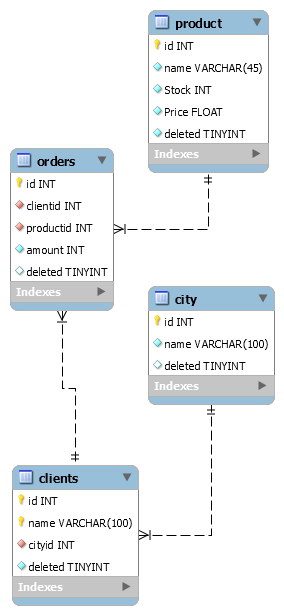
\includegraphics[scale=0.50]{DBModel.png}
\caption{Database Diagram for the Warehouse}
\end{figure}
\FloatBarrier
\pagebreak
\subsection{Command Syntax}
In order to process the commands from the text file a parser has to be implemented in order to process the commands and those commands have to follow a specific syntax in order to be recognized correctly.
\subsubsection{Add client}
Syntax: Insert client: Ion Popescu, Bucuresti\par
Description: Inserts into the database a new client with name Ion Popescu and address Bucuresti
\subsubsection{Add product}
Syntax: Insert product: apple, 20, 1\par
Description: Inserts into the database a new product called apple with quantity 20 and price 1
\subsubsection{Delete product}
Syntax: Delete product: apple\par
Description: Deletes the product apple from the database
\subsubsection{Delete client}
Syntax: Delete client: Ion Popescui\par
Description: Deletes the client with name Ion Popescu from the database.
\subsubsection{Create order for client}
Syntax: Order: Ion Popescu, apple, 5
Description: Creates a new order for Ion Popescu with apple quantity 5. It decrements the apple stock by 5 and generates a bill for it.Each order command represents a new order
\subsubsection{Generate Reports}
Syntax: Report client/order/product
Description: Generates a new report with all clients/orders/products.
\pagebreak
\subsection{Class Design}
The class structure of this program follows a layered architecture which consists of splitting the application into different layers, each with its own specific purpose and calls functions from below it
\begin{figure}[!htb]
\centering
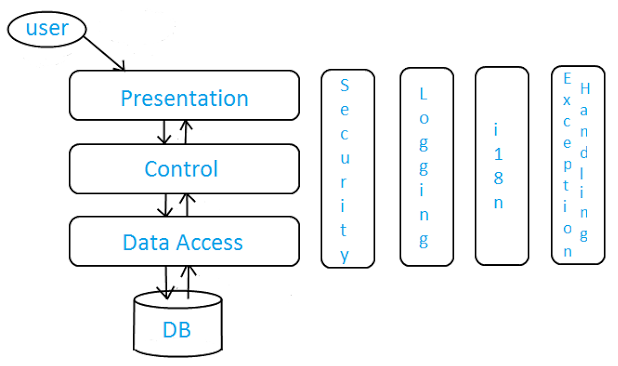
\includegraphics[scale=0.40]{layers.png}
\caption{Example of a layered architecture}
\end{figure}
\FloatBarrier
UML, short for Unified Modeling Language, is a standardized modeling language consisting of an integrated set of diagrams, developed to help system and software developers for specifying, visualizing, constructing, and documenting the artifacts of software systems. It allows us to visualize the class structure of the three aforementioned packages and how they interact with each other.\par
\begin{figure}[!htb]
\centering
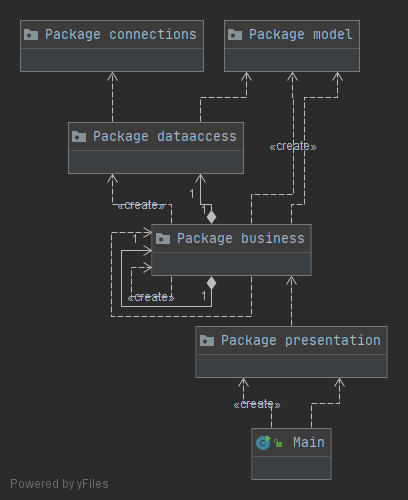
\includegraphics[scale=0.40]{package_struct.png}
\caption{Package structure of my application}
\end{figure}
\FloatBarrier
\begin{figure}[!htb]
\centering
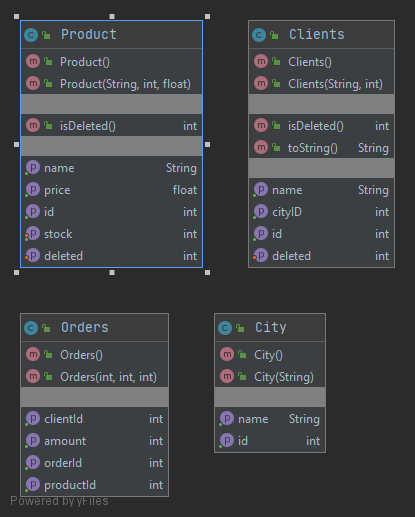
\includegraphics[scale=0.40]{model.png}
\caption{Model package}
\end{figure}
\FloatBarrier
\begin{figure}[!htb]
\centering
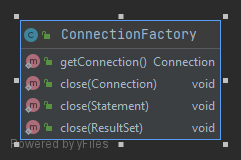
\includegraphics[scale=0.40]{connections.png}
\caption{Connections package}
\end{figure}
\FloatBarrier
\begin{figure}[!htb]
\centering
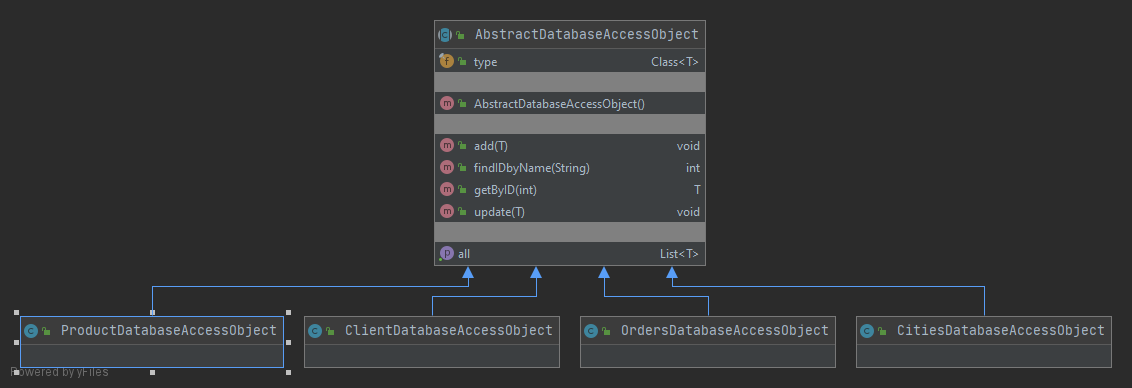
\includegraphics[scale=0.40]{dataaccess.png}
\caption{Data access package}
\end{figure}
\FloatBarrier
\begin{figure}[!htb]
\centering
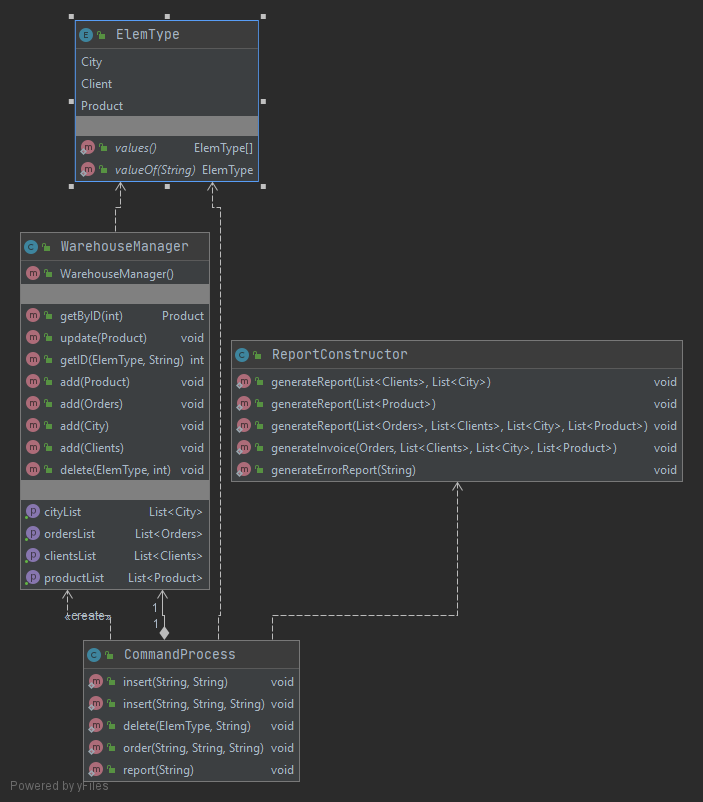
\includegraphics[scale=0.40]{business.png}
\caption{Business package}
\end{figure}
\FloatBarrier
\begin{figure}[!htb]
\centering
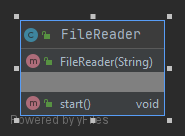
\includegraphics[scale=0.40]{presentation.png}
\caption{Presentation package}
\end{figure}
\FloatBarrier
\pagebreak
\section{Implementation}
This chapter will describe all classes which make up the application.

\subsection{Connections}
The Connections package provides the singleton class ConnectionFactory which provides static methods to create and close connections between the application and the DBMS.
\subsubsection{getConnection}
Creates a new connection to the database or fetches an existing one and returns it.
\subsubsection{close(Connection/ResultSet/Statement)}
Overloaded method which closes the Connection/ResultSet/Statement given in the argument.

\subsection{AbstractDatabaseAccessObject}
This is an abstract class which provides the genertic CRUD operations which are generated using generic classes and reflection techniques in order to select the proper table and get the necessary fields. This class' methods will be inherited by the other classes in the dataaccess package.
\subsubsection{add(T)}
Method to add the generic model paramenter to its corresponding table in the database using reflection methods. It creates the Insertion query inserts the data necessary to complete it such as the name of the table,fields to be filled and their corresponding data.
\subsubsection{findIDbyName(String name)}
Method to find an entry in the database based on its name, it will not work with all tables but its useful for finding clients or products based on their names. It returns their id in the database.
\subsubsection{getByID(int id)}
Fetches the model from the database based on its id. It returns null if it doesn't find it.
\subsubsection{getALL()}
Returns a list of all elements in one table, the table is dependent on the class which inherited this method
\subsubsection{update(T)}
Updates an entry in the database based on the id inside the generic T element.

\subsection{ClientDatabaseAccessObject}
This class provides the necessary methods to process all database access regarding the client table. It gets its methods from the abstract class which has the generic parameter a Client class.

\subsection{CitiesDatabaseAccessObject}
This class provides the necessary methods to process all database access regarding the Cities table. It inherits those methods from the abstract class which has the generic parameter a Cities class.

\subsection{ProductDatabaseAccessObject}
This class provides the necessary methods to process all database access regarding the product table. It uses the methods implemented in the abstract class but with a Product class as the generic parameter.

\subsection{OrdersDatabaseAccessObject}
This class provides the necessary methods to process all database access regarding the orders table. Like all classes in the dataaccess package it inherits its methods from the abstract class AbstractDatabaseAccessObject and has the Order class as its generic parameter.

\subsection{City}
It provides the necessary data structure and methods to represent an entry in the city table
\subsubsection{Important fields}
\begin{itemize}
\item id - id inside the table
\item Name - name of the city
\end{itemize}
\subsubsection{getName()}
Gets the name of the city.
\subsubsection{getID()}
Fetches the id of the city.

\subsection{Clients}
It provides the necessary data structure and methods to represent an entry in the clients table
\subsubsection{Important fields}
\begin{itemize}
\item id - id inside the table
\item Name - name of the client
\item cityID - city identifier inside the table
\item deleted - flag to check if the client was previously deleted or not
\end{itemize}
\subsubsection{getName()}
Gets the name of the client.
\subsubsection{getID()}
Fetches the id of the client.
\subsubsection{getCityID()}
Fetches the id of the city the client resides in.
\subsubsection{isDeleted()}
Checks if the client was deleted or not.
\subsubsection{setDeleted()}
Sets the deleted flag to the value in the parameter.

\subsection{Product}
It provides the necessary data structure and methods to represent an entry in the products table
\subsubsection{Important fields}
\begin{itemize}
\item id - id inside the table
\item Name - name of the product
\item stock - amount of product currently in stock
\item price - price of the product
\item deleted - flag to check if the client was previously deleted or not
\end{itemize}
\subsubsection{getName()}
Gets the name of the product.
\subsubsection{getID()}
Fetches the id of the product.
\subsubsection{setStock()}
Updates the stock of the product.
\subsubsection{getStock()}
Gets the amount of product currently in stock.
\subsubsection{getPrice()}
Fetches the price of the product.
\subsubsection{isDeleted()}
Checks if the client was deleted or not.
\subsubsection{setDeleted()}
Sets the deleted flag to the value in the parameter.

\subsection{Orders}
It provides the necessary data structure and methods to represent an entry in the orders table
\subsubsection{Important fields}
\begin{itemize}
\item id - id inside the table
\item clientId - id of the client who placed the order
\item productId - id of the product ordered
\item amount - amount of product ordered
\end{itemize}
\subsubsection{getOrderID()}
Gets the id of the order
\subsubsection{getClientID()}
Fetches the id of the client who ordered the product.
\subsubsection{getProductID()}
Fetches the id of the ordered product.
\subsubsection{getAmount()}
Fetches the id of the amount ordered.

\subsection{CommandProcess}
Wrapper to process the commands further in order to pass them to the Warehouse Manger and actually add them to the DB.
\subsubsection{insert()}
Inserts a new client or product depending on the number of arguments. It translates them into their corresponding Model object and sends it to the WarehouseManager instance.
\subsubsection{delete()}
Deletes an entry from the database based on the type and name of the entity deleted. It finds the id and passes a delete command
\subsubsection{order()}
Creates a new order based on the name of client,name of product,amount of product. Queries the product and client tables to get their ids, checks the available stock and adds it if there is enough it adds it to the database and generates an invoice or creates an error report.
\subsubsection{report()}
Determines which kind of report to create and passes it to the ReportConstructor class.

\subsection{ReportConstructor}
Provides static methods to create reports and invoices pdf files using the iText library.
\subsubsection{generateErrorReport(String message)}
Creates an error report with the specified error message.
\subsubsection{generateInvoice()}
Creates a new invoice based of the order object passed as an argument.
\subsubsection{generateReport()}
Overloaded method which generates a new report based on the number of lists given(1 for Product, 2 for clients,4 for orders).
\subsection{WarehouseManager}
Class which composes all DAOs and provides methods to interact with them and perform the CRUD operations.
\subsection{ElemType}
Enum needed to decode which kind of element(City,Client or Product) is needed to be fetched. Used by WarehoudeManager and CommandProcess.
\subsection{FileReader}
It opens a file scanner and reads line by line and processes the commands like this:
\begin{figure}[!htb]
\centering
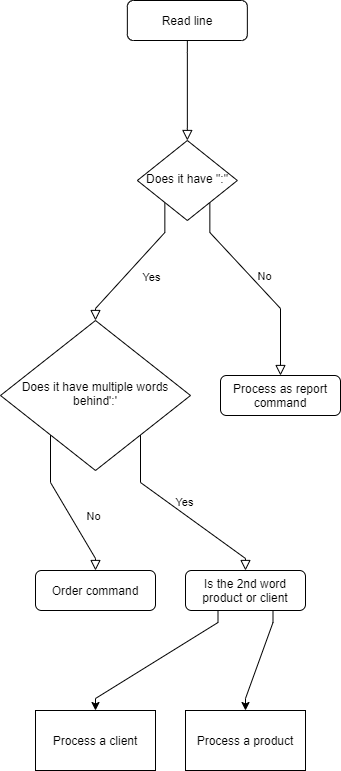
\includegraphics[scale=0.60]{diagram.png}
\caption{Decision tree of the FileReader}
\end{figure}
\FloatBarrier
\section{Testing}
There was a basic command list that had to be run and provide its output inside the repository. The file basically tests if the elements from the database are inserted and removed properly, that error conditions that may arise from the order command(such as out of stock errors) are properly handled.
\begin{verbatim}
Insert client: Ion Popescu, Bucuresti
Insert client: Luca George, Bucuresti
Report client
Insert client: Sandu Vasile, Cluj-Napoca
Report client
Delete client: Ion Popescu, Bucuresti
Report client
Insert product: apple, 20, 1
Insert product: peach, 50, 2
Insert product: apple, 20, 1
Report product
Delete Product: peach
Insert product: orange, 40, 1.5
Insert product: lemon, 70, 2
Report product
Order: Luca George, apple, 5
Order: Luca George, lemon, 5
Order: Sandu Vasile, apple, 100
Report client
Report order
Report product
\end{verbatim}
\section{Conclusions}
This assignment is a great usage of the Layered architecture in Java OOP design and it highly encourages the programmer to use Reflection techniques to optimize the design and code bloat while also introducing the programmer to libraries such as iText and the MySQL connector.
\section{Bibliography}
\begin{itemize}
\item http://www.mkyong.com/jdbc/how-to-connect-to-mysql-with-jdbc-driver-java/
\item http://theopentutorials.com/tutorials/java/jdbc/jdbc-mysql-create-database-example
\item https://dzone.com/articles/layers-standard-enterprise
\item http://tutorials.jenkov.com/java-reflection/index.htm
\item https://www.baeldung.com/java-pdf-creation
\item https://www.baeldung.com/javadoc

\end{itemize}
\end{document}